
\section{Metode Runge-Kutta Adaptif\label{sec:Adaptive-Runge-Kutta-Methods}\index{metode Runge-Kutta}\index{metode Runge-Kutta adaptif}\index{metode!Runge-Kutta adaptif|see {metode Runge-Kutta adaptif}}}

\renewcommand{\arraystretch}{1.4}Dua pemecah PDB yang diturunkan
pada Bagian \ref{sec:Runge-Kutta-Methods} menggunakan rangkaian perhitungan
yang persis sama untuk $k_{1}$, $k_{2}$, dan $k_{3}$, tetapi menggabungkan
hasilnya secara berbeda untuk menghitung $y_{i+1}$. Pada saat itu,
keduanya disebut PDB-terbuka dan PDB-tertutup-terbuka. Dalam analisis
pada Bagian \ref{sec:Runge-Kutta-Error-Analysis} disebutkan bahwa
PDB-terbuka bukan metode yang efisien, sedangkan PDB-tertutup-terbuka
efisien; sejak saat itu kita mulai menyebut PDB-tertutup-terbuka dengan
nama yang sebenarnya, metode orde ketiga Heun. 

\noindent\begin{digression}{Metode orde ketiga Heun}\index{metode orde ketiga Heun}

\noindent Dalam artikel tahun 1900 ini \cite{heun} Karl Heun\index{Heun!Karl}
mengemukakan metode orde ketiga yang menyandang namanya. Meskipun
Anda tidak dapat membaca bahasa Jerman, rumus VI)-nya jelas!

\begin{center}
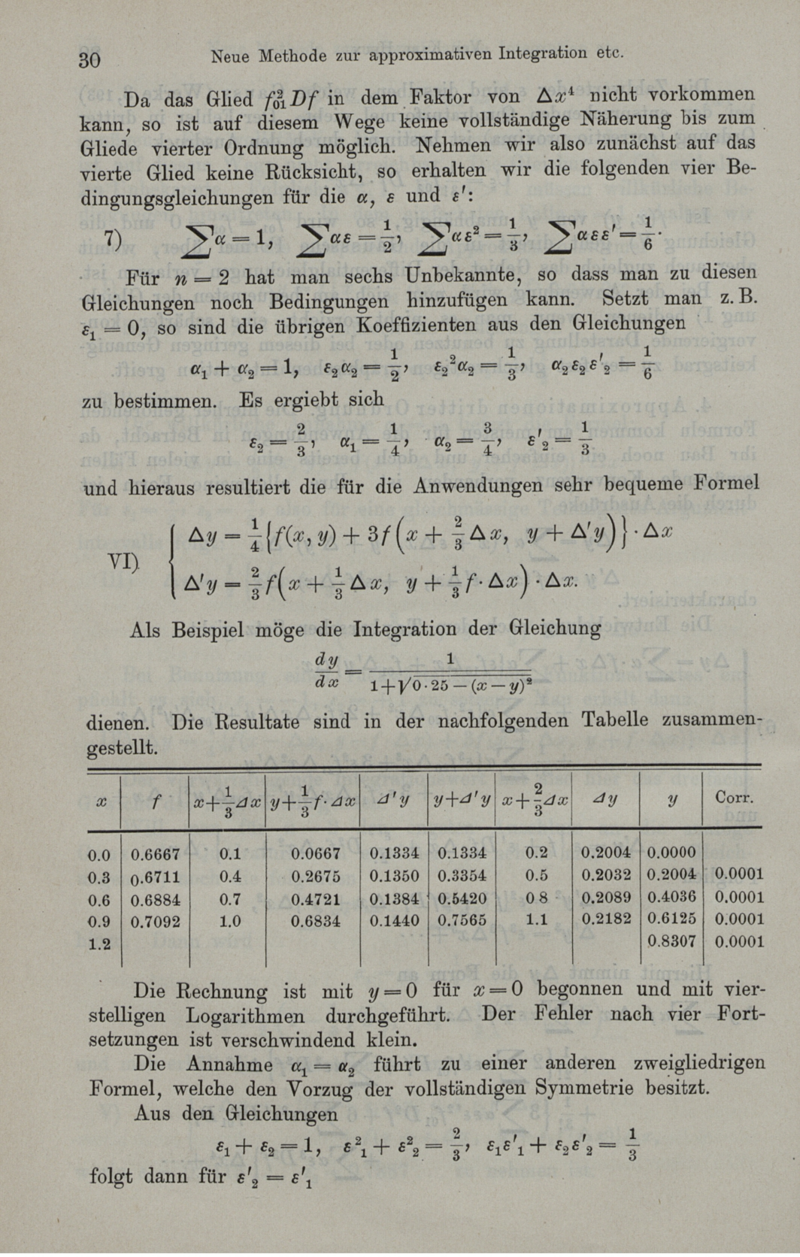
\includegraphics{references/heun1900/00000036}
\par\end{center}

\noindent\end{digression}

\noindent Karena tidak efisien, PDB-terbuka tidak boleh digunakan
sendiri dalam praktik, tetapi jika digabungkan dengan metode orde
ketiga Heun, metode ini memiliki potensi kegunaan.

Menurut metode orde ketiga Heun
\begin{eqnarray*}
k_{1} & = & f(t_{i},y_{i})\\
k_{2} & = & f\left(t_{i}+\frac{h}{3},y_{i}+\frac{h}{3}k_{1}\right)\\
k_{3} & = & f\left(t_{i}+\frac{2h}{3},y_{i}+\frac{2h}{3}k_{2}\right)\\
y_{i+1} & = & y_{i}+\frac{h}{4}\left[k_{1}+3k_{3}\right]+O(h^{4}).
\end{eqnarray*}
Dengan menggunakan nilai $k_{1}$, $k_{2}$, dan $k_{3}$, metode
PDB-terbuka dihitung sebagai
\[
y_{i+1}=y_{i}+\frac{h}{2}\left[k_{2}+k_{3}\right]+O(h^{3}).
\]
Selisih antara kedua taksiran ini adalah
\begin{equation}
\frac{h}{4}\left[k_{1}-2k_{2}+k_{3}\right]=Mh^{3}+O(h^{4})\label{eq:heunAdaptiveError}
\end{equation}
untuk suatu konstanta $M$, dan menyatakan galat pemenggalan lokal
metode berorde lebih rendah, PDB-terbuka. Taksiran galat ini dapat
digunakan untuk menyesuaikan nilai $h$ dari satu langkah ke langkah
berikutnya, dengan memperkecil ukuran langkah ketika galat pemenggalan
lokal lebih besar daripada suatu toleransi dan memperbesar ukuran
langkah ketika galat pemenggalan lokal lebih kecil daripada toleransi
tersebut.

Untuk mengilustrasikan algoritme dan manfaat rutin adaptif, mari kita
kembali ke PDB \ref{eq:sampleODE}, $\dot{y}=-\frac{y}{t}+t^{2}$,
yang sudah berulang kali kita manfaatkan. Seperti sebelumnya, kita
akan menaksir $y(2)$ dengan kondisi awal $y(4)=20$. Kali ini jumlah
langkah yang akan dihitung ditentukan oleh algoritme, bukan oleh kita,
setidaknya setelah langkah pertama. Sayangnya, tidak ada cara baku
atau yang sepenuhnya andal untuk memilih ukuran langkah pertama. Karena
kita mencari perhitungan yang dapat dilakukan dengan tangan, mari
kita coba $h=-1$ sebagai permulaan, yaitu $\frac{1}{2}$ dari lebar
interval $[2,4]$ tempat kita akan melakukan integrasi. 

Seperti pada kuadratur adaptif, tingkat akurasi yang diinginkan, atau
toleransi, juga diperlukan di sini. Sekali lagi, karena kita mencari
perhitungan yang dapat dilakukan dengan tangan, mari kita coba $0.1$,
tingkat akurasi yang cukup sederhana. Akhirnya, kita siap menghitung:
\begin{eqnarray*}
k_{1} & = & f(4,20)=11\\
k_{2} & = & f\left(4-\frac{1}{3},20-\frac{1}{3}\cdot11\right)\approx8.98989898989899\\
k_{3} & = & f\left(4-\frac{2}{3},20-\frac{2}{3}\cdot8.9898\ldots\right)\approx6.90909090909091.
\end{eqnarray*}
Sebelum menghitung $y_{1}$ dari nilai-nilai ini, kita perlu memastikan
bahwa taksiran galat perhitungan tidak melampaui batas $0.1$:
\[
\left|\frac{h}{4}\left[k_{1}-2k_{2}+k_{3}\right]\right|\approx0.017.
\]
Taksiran galat untuk langkah menuju $t_{1}=3$ adalah sekitar $0.02$,
jauh di bawah ambang yang diinginkan. Kita dapat melanjutkan:
\begin{eqnarray*}
y_{1} & = & y_{0}+\frac{h}{4}\left[k_{1}+3k_{3}\right]\approx12.06818181818182\\
t_{1} & = & t_{0}+h=3.
\end{eqnarray*}
Dengan demikian, kita memperoleh $y(3)\approx12.07$. Dengan melanjutkan
menggunakan $h=1$,
\begin{eqnarray*}
k_{1} & = & f(3,12.068\ldots)\approx4.977272727272728\\
k_{2} & = & f\left(3-\frac{1}{3},12.068\ldots-\frac{1}{3}\cdot4.9773\ldots\right)\approx3.20770202020202\\
k_{3} & = & f\left(3-\frac{2}{3},12.068\ldots-\frac{2}{3}\cdot3.2077\ldots\right)\approx1.188852813852814.
\end{eqnarray*}
Sebelum menghitung $y_{2}$ dari nilai-nilai ini, kita perlu memastikan
bahwa taksiran galat perhitungan tidak melampaui batas $0.1$:
\[
\left|\frac{h}{4}\left[k_{1}-2k_{2}+k_{3}\right]\right|\approx0.062.
\]
Taksiran galat untuk langkah menuju $t_{2}=2$ adalah sekitar $0.06$,
jauh di bawah ambang yang diinginkan. Kita dapat melanjutkan:
\begin{eqnarray*}
y_{2} & = & y_{1}+\frac{h}{4}\left[k_{1}+3k_{3}\right]\approx9.932224025974026\\
t_{1} & = & t_{0}+h=2.
\end{eqnarray*}
Dengan demikian, kita memperoleh $y(2)\approx9.932$. Setelah dua
langkah, galat sebenarnya adalah sekitar $|10-9.932|=0.068$. Tentu
saja, kita bisa saja langsung menerapkan metode orde ketiga Heun dengan
ukuran langkah $h=1$ (tanpa pemeriksaan galat) dan memperoleh jawaban
yang sama. Perbedaannya adalah kita sama sekali tidak tahu seberapa
besar galat yang akan terjadi! Dengan metode adaptif, Anda dapat cukup
yakin bahwa setiap langkah menimbulkan galat sebesar yang Anda minta.
Untuk menegaskan hal ini sekali lagi, pertimbangkan mengulang perhitungan
dengan ukuran langkah $h=-2$:
\begin{eqnarray*}
k_{1} & = & f(4,20)=11\\
k_{2} & = & f\left(4-\frac{2}{3},20-\frac{2}{3}\cdot11\right)\approx7.311111111111111\\
k_{3} & = & f\left(4-\frac{4}{3},20-\frac{4}{3}\cdot7.3111\ldots\right)\approx3.266666666666667.
\end{eqnarray*}
Jika kita melanjutkan dengan metode orde ketiga Heun (tanpa pemeriksaan
galat), kita memperoleh
\begin{eqnarray*}
y_{1} & = & y_{0}+\frac{h}{4}\left[k_{1}+3k_{3}\right]\approx9.6\\
t_{1} & = & t_{0}+h=2.
\end{eqnarray*}
Namun, tanpa jawaban eksak, sebagaimana lazimnya ketika menggunakan
metode numerik, kita tidak dapat mengetahui seberapa akurat taksiran
ini! Dalam hal itu, nilai $9.6$ merupakan taksiran yang kurang berguna.

Di sisi lain, karena kita mengetahui nilai eksak $y(2)$ adalah 10,
kita tahu galatnya $0.4$, lebih besar daripada nilai $0.1$. Metode
Heun adaptif seharusnya mendeteksi hal ini dan menghasilkan taksiran
yang lebih akurat:
\[
\left|\frac{h}{4}\left[k_{1}-2k_{2}+k_{3}\right]\right|\approx0.177.
\]
Metode adaptif akan menolak langkah ini karena taksiran galat lebih
besar daripada akurasi yang diinginkan, tanpa menghitung $y_{1}$!
Jadi, apa yang harus dilakukan? Metode adaptif akan mencoba lagi dengan
ukuran langkah yang lebih kecil.

Karena 
\[
\left|\frac{h}{4}\left[k_{1}-2k_{2}+k_{3}\right]\right|\approx Mh^{3},
\]
kita memiliki $Mh^{3}\approx0.177$ untuk setiap ukuran langkah yang
dekat dengan ukuran yang baru dicoba. Jika ukuran langkah diskalakan
dengan faktor $q$, taksiran galat baru seharusnya sekitar $M(qh)^{3}$,
atau $q^{3}Mh^{3}\approx0.177q^{3}$. Karena kita menginginkan galat
tersebut tidak lebih dari $0.1$, kita harus memilih $q$ sedemikian
sehingga $0.177q^{3}<0.1$ atau $q^{3}<\frac{0.1}{0.177}$, yang menyiratkan
$q<\sqrt[3]{\frac{0.1}{0.177}}\approx0.8254$. Namun, algoritme akan
sangat melambat jika ukuran langkah terlalu sering menjadi terlalu
besar; karena itu, kita memilih langkah berikut yang agak konservatif,
yaitu sebesar $0.9qh\approx0.9(0.8254)(-2)\approx-1.485$. Menghitung
ulang dengan ukuran langkah baru:
\begin{eqnarray*}
k_{1} & = & f(4,20)=11\\
k_{2} & = & f\left(4-\frac{1.485}{3},20-\frac{1.485}{3}\cdot11\right)\approx8.130924301356263\\
k_{3} & = & f\left(4-\frac{4}{3},20-\frac{4}{3}\cdot7.3111\ldots\right)\approx5.087191526760124.
\end{eqnarray*}
dan
\[
\left|\frac{h}{4}\left[k_{1}-2k_{2}+k_{3}\right]\right|\approx0.06487930780869297,
\]
sehingga langkah ini diterima:
\begin{eqnarray*}
y_{2} & = & y_{1}+\frac{h}{4}\left[k_{1}+3k_{3}\right]\approx10.24469652063055\\
t_{1} & = & t_{0}+h=2.514132737997418.
\end{eqnarray*}
Sekarang kita mempertahankan ukuran langkah baru sampai terbukti tidak
sesuai. Dalam kasus ini, hal itu langsung terjadi. Langkah lain sebesar
$-1.485$ akan membawa solusi ke $t_{2}\approx1.028$, jauh melewati
nilai $t=2$. Jadi, kita memperpendek ukuran langkah menjadi $2-t_{1}=-0.514132737997418$.
Tidak perlu khawatir memperpendek ukuran langkah karena hal itu diperkirakan
akan mengurangi galat! Akhirnya, dengan $h=-0.514132737997418$:
\begin{eqnarray*}
k_{1} & = & f(2.514\ldots,10.244\ldots)\approx2.246020292164824\\
k_{2} & = & f\left(2.514\ldots-\frac{0.5141\ldots}{3},10.244\ldots-2\frac{0.5141\ldots}{3}\cdot2.246\ldots\right)\approx1.279876276642283\\
k_{3} & = & f\left(2.514\ldots-\frac{0.5141\ldots}{3},10.244\ldots-2\frac{0.5141\ldots}{3}\cdot1.279\ldots\right)\approx0.1988478127940674.
\end{eqnarray*}
dan 
\[
\left|\frac{h}{4}\left[k_{1}-2k_{2}+k_{3}\right]\right|\approx0.01476646399275057,
\]
langkah ini diterima:
\begin{eqnarray*}
y_{2} & = & y_{1}+\frac{h}{4}\left[k_{1}+3k_{3}\right]\approx9.879332752200975\\
t_{1} & = & t_{0}+h=2.
\end{eqnarray*}
Kita memperoleh $y(2)\approx9.879332752200975$ dan cukup yakin bahwa
galatnya tidak akan jauh melebihi nilai sekitar $0.2$, karena kita
mengambil dua langkah yang masing-masing mungkin menimbulkan galat
sekitar $0.1$. Tidak ada jaminan galatnya akan kurang dari $0.2$,
tetapi setidaknya kita cukup yakin bahwa nilainya tidak jauh lebih
besar. Karena kita menggunakan taksiran ukuran langkah yang konservatif,
galat sebenarnya mungkin sedikit lebih kecil (ternyata galatnya sekitar
0,12).

\subsection{Runge-Kutta Adaptif (kode semu)\index{metode Runge-Kutta adaptif!kode semu}}

Ada banyak skema Runge-Kutta adaptif, tetapi skema yang dibahas di
sini menggunakan metode orde kedua dan ketiga, sehingga dapat disebut
RK2(3).\index{metode RK2(3)} Secara teknis, ini adalah metode orde
2 karena taksiran galatnya berlaku untuk metode berorde lebih rendah.
Namun, dalam praktik, sering kali metode berorde lebih tinggi yang
digunakan untuk solusi PDB. Meskipun tidak ada jaminan bahwa metode
berorde lebih tinggi lebih akurat daripada metode berorde lebih rendah,
hal itu jarang menimbulkan masalah serius. Selain menggunakan faktor
keamanan sebesar $0.9$ ketika menyesuaikan ukuran langkah, kita juga
tidak mengizinkan penskalaan terhadap $h$ dengan faktor kurang dari
$0.1$ atau faktor lebih dari $5$. Pembatas tambahan ini tidak terlalu
ketat karena tetap memungkinkan pertumbuhan atau peluruhan eksponensial
$h$, tetapi dapat membantu menghindari masalah ketika taksiran galat
memang buruk. Selain itu, taksiran tersebut hanya akurat dalam rentang
sempit karena konstanta proporsionalitas dapat berubah drastis akibat
perubahan besar pada $h$. Pembahasan algoritme yang lebih terperinci
dapat ditemukan dalam \cite{recipes} Bagian 16.2.

\noindent\begin{pseudocode} 
\begin{description}
\item [{Asumsi:}] $\dot{y}=f(t,y)$, $y(a)=y_{0}$ memiliki solusi unik
pada interval dari $a$ hingga $b$.
\item [{Masukan:}] Nilai awal $(a,y_{0})$; fungsi $f(t,y)$; titik-titik
ujung interval, $a$ dan $b$; ukuran langkah awal $h$; akurasi yang
diinginkan $tol$; jumlah maksimum iterasi $N$.
\item [{Langkah~1:}] Tetapkan $i=1$; $t=a$; $y=y_{0}$; $\mbox{selesai}=false$;
\item [{Langkah~2:}] Selama $\mbox{belum selesai}\mbox{ dan }i\leq N$
lakukan Langkah 3--6:

\begin{description}
\item [{Langkah~3:}] Jika $((b-(t+h))\cdot(b-a)\leq0)$ maka tetapkan
$h=b-t$; $\mbox{selesai}=true$;
\item [{Langkah~4:}] Tetapkan $k_{1}=f(t,y)$; $k_{2}=f(t+\frac{h}{3},y+\frac{h}{3}k_{1})$;
$k_{3}=f(t+\frac{2h}{3},y+\frac{2h}{3}k_{2})$; $\mbox{err}=|\frac{h}{4}(k_{1}-2k_{2}+k_{3})|$;
\item [{Langkah~5:}] Jika selesai atau $\mbox{err}\leq tol$ maka tetapkan
$y=y+\frac{h}{4}(k_{1}+3k_{3})$; $\mbox{temp}=t+h$;
\item [{Langkah~6:}] Jika $\mbox{temp}=t$ maka lakukan Langkah 7--8:

\begin{description}
\item [{Langkah~7:}] Cetak ``Metode gagal. Ukuran langkah mencapai nol.''
\item [{Langkah~8:}] Kembali
\end{description}
\item [{Langkah~9:}] Tetapkan $i=i+1$;
\item [{Langkah~10:}] Jika $\mbox{err}<\frac{\mbox{tol}}{5}$ atau $\mbox{err}>\mbox{tol}$
maka lakukan Langkah 11--14:

\begin{description}
\item [{Langkah~11:}] Tetapkan $q=0.9\left(\frac{\mbox{tol}}{\mbox{err}}\right)^{\frac{1}{3}}$
\item [{Langkah~12:}] Jika $q<\frac{1}{10}$ maka tetapkan $q=\frac{1}{10}$
\item [{Langkah~13:}] Jika $q>5$ maka tetapkan $q=5$
\item [{Langkah~14:}] Tetapkan $h=qh$
\end{description}
\end{description}
\item [{Langkah~15:}] Jika belum selesai, cetak ``Metode gagal. Jumlah
iterasi maksimum terlampaui.''
\item [{Keluaran:}] Hampiran $y(b)$ atau pesan kegagalan.
\end{description}
\end{pseudocode}  

\noindent Rumus untuk $k_{i}$ dan err perlu diubah untuk skema Runge-Kutta
adaptif yang berbeda, begitu pula perhitungan ulang $h$ pada Langkah
11--14, tetapi algoritme dasarnya tidak perlu dimodifikasi untuk
metode tertanam lainnya.

\subsection{Skema Runge-Kutta Umum}

Sejauh ini, kita telah membahas metode Runge-Kutta berbentuk (\ref{eq:rungeKuttaGeneral}),
yang disalin di sini agar mudah dirujuk:
\begin{eqnarray*}
k_{1} & = & f(t_{i},y_{i})\\
k_{2} & = & f\left(t_{i}+\beta_{2}h,y_{i}+\beta_{2}hk_{1}\right)\\
k_{3} & = & f(t_{i}+\beta_{3}h,y_{i}+\beta_{3}hk_{2})\\
 & \vdots\\
k_{s} & = & f(t_{i}+\beta_{s}h,y_{i}+\beta_{s}hk_{s-1})\\
y_{i+1} & = & y_{i}+h\left[\alpha_{1}k_{1}+\alpha_{2}k_{2}+\alpha_{3}k_{3}+\cdots+\alpha_{s}k_{s}\right].
\end{eqnarray*}
Dalam metode jenis ini, $k_{1}$ digunakan dalam perhitungan $k_{2}$;
$k_{2}$ digunakan dalam perhitungan $k_{3}$; $k_{3}$ digunakan
dalam perhitungan $k_{4}$; dan seterusnya. Namun, tidak ada yang
menghalangi kita menurunkan metode yang menggunakan $k_{1}$ dan $k_{2}$
digunakan dalam perhitungan $k_{3}$; semua $k_{1}$, $k_{2}$, dan
$k_{3}$ digunakan dalam perhitungan $k_{4}$; dan secara umum, mengizinkan
semua $k_{1},k_{2},\ldots,k_{j-1}$ digunakan untuk menghitung $k_{j}$.
Hal itu memberikan lebih banyak derajat kebebasan untuk memenuhi persamaan
analisis galat, sehingga membuka kemungkinan adanya jauh lebih banyak
metode Runge-Kutta. Setiap metode dalam bentuk yang lebih umum ini
disebut metode Runge-Kutta eksplisit dan dapat dirumuskan sebagai
\begin{eqnarray}
k_{1} & = & f(t_{i},y_{i})\nonumber \\
k_{2} & = & f\left(t_{i}+\delta_{2}h,y_{i}+\beta_{21}hk_{1}\right)\nonumber \\
k_{3} & = & f(t_{i}+\delta_{3}h,y_{i}+\beta_{31}hk_{1}+\beta_{32}hk_{2})\nonumber \\
 & \vdots\nonumber \\
k_{s} & = & f(t_{i}+\delta_{s}h,y_{i}+\sum_{j=1}^{s-1}\beta_{sj}hk_{j})\nonumber \\
y_{i+1} & = & y_{i}+h\left[\alpha_{1}k_{1}+\alpha_{2}k_{2}+\alpha_{3}k_{3}+\cdots+\alpha_{s}k_{s}\right].\label{eq:Runge-Kutta-explicit}
\end{eqnarray}
Metode berbentuk ini sering diringkas dalam tableau Butcher,\index{Butcher tableau}

\begin{center}
\begin{tabular}{c|ccccc}
0 &  &  &  &  & \tabularnewline
$\delta_{2}$ & $\beta_{21}$ &  &  &  & \tabularnewline
$\delta_{3}$ & $\beta_{31}$ & $\beta_{32}$ &  &  & \tabularnewline
$\vdots$ & $\vdots$ &  & $\ddots$ &  & \tabularnewline
$\delta_{s}$ & $\beta_{s1}$ & $\beta_{s2}$ & $\cdots$ & $\beta_{s(s-1)}$ & \tabularnewline
\hline 
 & $\alpha_{1}$ & $\alpha_{2}$ & $\cdots$ & $\alpha_{s-1}$ & $\alpha_{s}$\tabularnewline
\end{tabular}
\par\end{center}

\noindent seperti koefisien sistem persamaan linear dapat diringkas
dalam sebuah matriks. Tableau Butcher untuk setiap metode Runge-Kutta
yang telah kita bahas sejauh ini akan berbentuk

\begin{center}
\begin{tabular}{c|cccccc}
0 &  &  &  &  &  & \tabularnewline
$\delta_{2}$ & $\beta_{21}$ &  &  &  &  & \tabularnewline
$\delta_{3}$ & 0 & $\beta_{32}$ &  &  &  & \tabularnewline
$\delta_{4}$ & 0 & 0 & $\beta_{43}$ &  &  & \tabularnewline
$\vdots$ & $\vdots$ & $\vdots$ & $\ddots$ & $\ddots$ &  & \tabularnewline
$\delta_{s}$ & 0 & 0 & $\cdots$ & 0 & $\beta_{s(s-1)}$ & \tabularnewline
\hline 
 & $\alpha_{1}$ & $\alpha_{2}$ & $\alpha_{3}$ & $\cdots$ & $\alpha_{s-1}$ & $\alpha_{s}$\tabularnewline
\end{tabular}
\par\end{center}

\noindent Sebagai contoh, metode orde ketiga Heun diringkas dalam
tableau Butcher sebagai

\begin{center}
\begin{tabular}{c|ccc}
0 &  &  & \tabularnewline
$\frac{1}{3}$ & $\frac{1}{3}$ &  & \tabularnewline
$\frac{2}{3}$ & 0 & $\frac{2}{3}$ & \tabularnewline
\hline 
 & $\frac{1}{4}$ & 0 & $\frac{3}{4}$\tabularnewline
\end{tabular}
\par\end{center}

\noindent Untuk keperluan kita, skema Runge-Kutta adaptif, yang juga
disebut metode tertanam, akan direpresentasikan dalam tableau Butcher
dengan menambahkan satu baris lagi untuk koefisien $\alpha_{j}$ metode
berorde lebih rendah. Sebagai contoh, tableau Butcher untuk RK2(3)
yang disajikan di atas adalah

\begin{center}
\begin{tabular}{c|ccc}
0 &  &  & \tabularnewline
$\frac{1}{3}$ & $\frac{1}{3}$ &  & \tabularnewline
$\frac{2}{3}$ & 0 & $\frac{2}{3}$ & \tabularnewline
\hline 
 & $\frac{1}{4}$ & 0 & $\frac{3}{4}$\tabularnewline
\hline 
 & 0 & $\frac{1}{2}$ & $\frac{1}{2}$\tabularnewline
\end{tabular}
\par\end{center}

\noindent Bentuk tableau Butcher paling umum untuk metode tak tertanam
adalah

\begin{center}
\begin{tabular}{c|cccc}
0 & $\beta_{11}$ & $\beta_{12}$ & $\cdots$ & $\beta_{1s}$\tabularnewline
$\delta_{2}$ & $\beta_{21}$ & $\beta_{22}$ & $\cdots$ & $\beta_{2s}$\tabularnewline
$\vdots$ & $\vdots$ & $\vdots$ & $\ddots$ & $\vdots$\tabularnewline
$\delta_{s}$ & $\beta_{s1}$ & $\beta_{s2}$ & $\cdots$ & $\beta_{ss}$\tabularnewline
\hline 
 & $\alpha_{1}$ & $\alpha_{2}$ & $\cdots$ & $\alpha_{s}$\tabularnewline
\end{tabular}
\par\end{center}

\noindent Jika salah satu $\beta_{ij}$ dengan $j>i$ tidak nol, skema
Runge-Kutta terkait merupakan metode implisit. Setiap langkah metode
ini memerlukan penyelesaian suatu sistem persamaan. Metode Runge-Kutta
implisit dapat digunakan untuk menghampiri solusi PDB kaku karena
metode eksplisit sering kali sangat buruk untuk tujuan tersebut.\index{metode Runge-Kutta implisit}\index{metode!Runge-Kutta implisit|see {metode Runge-Kutta implisit}}

\noindent\begin{digression}{Persamaan Diferensial Biasa Kaku}\index{persamaan diferensial!kaku}

\noindent Persamaan diferensial biasa
\begin{eqnarray}
\dot{x} & = & x^{2}-x^{3}\nonumber \\
x(0) & = & \delta\label{eq:stiffODE}
\end{eqnarray}
tidak memiliki solusi bentuk tertutup. Solusi implisit adalah hasil
terbaik yang dapat diturunkan, sehingga solusi numerik diperlukan
untuk menghampiri nilai fungsi. Namun, beberapa analisis dasar dapat
memberikan gambaran tentang sifat solusi tersebut. Persamaan ini memiliki
titik kesetimbangan di $x=0$, yang berarti bahwa jika $x(t_{0})=0$
untuk suatu $t_{0}$, maka $x(t)=0$ untuk semua $t$. Fungsi tersebut
tetap konstan sepanjang waktu. Fungsi tersebut berada dalam keadaan
setimbang. Fungsi tersebut tidak berubah. Hal ini mengikuti fakta
bahwa ketika $x=0$, $\dot{x}=0^{2}-0^{3}=0$. Demikian pula, PDB
memiliki titik kesetimbangan di $x=1$ (karena $1$ merupakan akar
lain dari polinom $x^{2}-x^{3}$), dan PDB tersebut tidak memiliki
titik kesetimbangan lain. Namun, kedua titik kesetimbangan itu sangat
berbeda satu sama lain. Titik kesetimbangan di $x=0$ bersifat tak
stabil, sedangkan titik kesetimbangan di $x=1$ bersifat stabil. Jika
$x(t_{0})$ cukup dekat dengan $1$ ($|x(t_{0})-1|<1$ sudah memadai),
maka $x$ akan menuju $1$ ketika $t\to\infty$. Namun, tidak ada
syarat seperti itu di sekitar $x=0$. Seberapa dekat pun $x(t_{0})$
dengan nol, jika nilainya positif, $x$ tetap akan menuju titik kesetimbangan
yang lain, yaitu $1$, ketika $t\to\infty$. Namun, yang lebih penting
adalah bagaimana nilai-nilai $x$ mendekati $1$ ketika $t\to\infty$. 

Harapan kita terhadap pemecah PDB adaptif adalah bahwa pemecah tersebut
akan mengambil langkah besar di daerah tempat fungsi tidak berubah
dengan cepat (memiliki turunan pertama yang kecil), serta lebih berhati-hati
dengan mengambil langkah kecil di daerah tempat fungsi berubah dengan
cepat (memiliki turunan pertama yang besar). Pada umumnya, inilah
yang terjadi. PDB kaku merupakan pengecualian: metode adaptif mengambil
banyak langkah kecil bahkan di daerah tempat fungsi memiliki turunan
pertama yang kecil. Gambar-gambar berikut menunjukkan solusi dari
(\ref{eq:stiffODE}) menggunakan RK2(3) dengan toleransi $10^{-6}$,
$\delta=10^{-3}$, dan ukuran langkah awal $3$ pada interval $[0,\frac{2}{\delta}]$.
Pertama, solusi pada $[0,980]$ berperilaku sesuai harapan. Pemecah
mengambil langkah besar, termasuk satu langkah dari $t\approx93$
hingga $t\approx210$, dengan ukuran langkah $h>117$ pada bagian
awal tempat fungsi berubah sangat lambat. 

\begin{center}
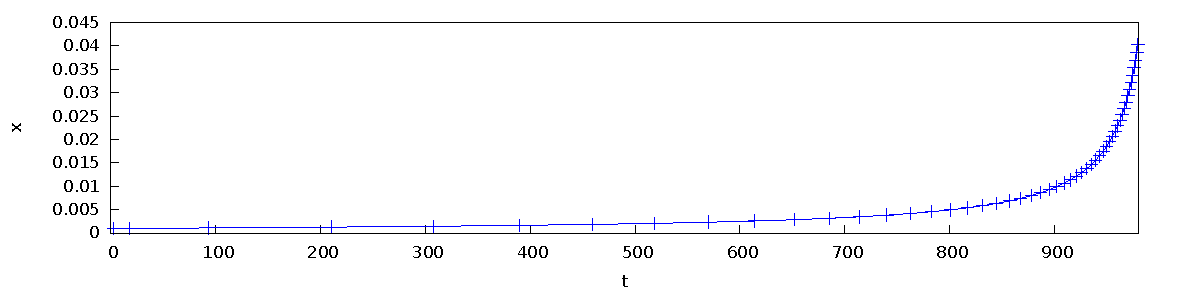
\includegraphics[width=6in]{figures/ode-stiffFrontEnd}
\par\end{center}

\noindent Di bagian tengah, solusi pada $[980,1020]$ tetap berperilaku
sesuai harapan. Di sini solusi mulai berubah lebih cepat sehingga
pemecah mengambil sejumlah langkah yang lebih kecil. 

\begin{center}
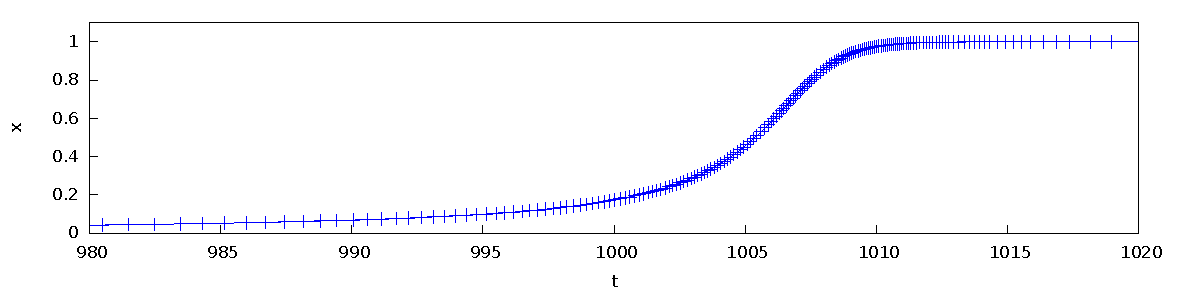
\includegraphics[width=6in]{figures/ode-stiffMiddle}
\par\end{center}

\noindent Menjelang akhir, solusi pada $[1020,2000]$ menunjukkan
akibat kekakuan. Solusi eksak hampir konstan di daerah ini dan secara
bertahap mendekati 1 dari bawah. Pemecah yang baik akan kembali mengambil
langkah besar melintasi daerah ini, tetapi skema Runge-Kutta eksplisit
yang adaptif tidak melakukannya. Solusi numerik berosilasi di sekitar
1 dalam batas toleransi, sehingga memang melakukan hal yang seharusnya,
tetapi memerlukan banyak langkah pendek untuk itu.

\begin{center}
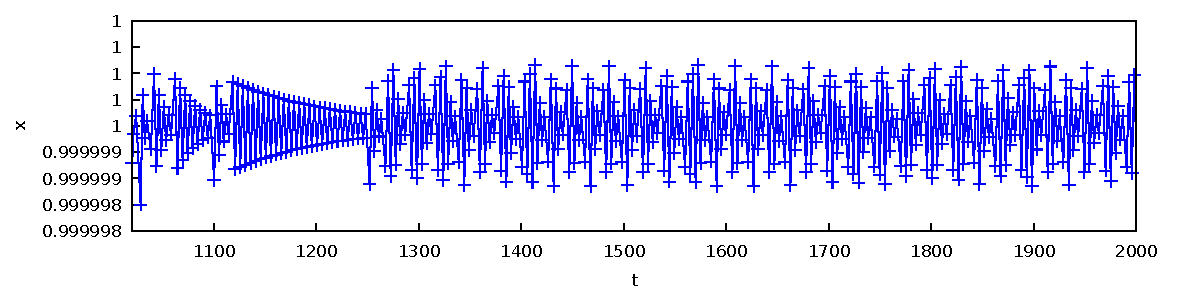
\includegraphics[width=6in]{figures/ode-stiffTailEnd}
\par\end{center}

\noindent\end{digression}

\subsection{Konsep Kunci}
\begin{description}
\item [{Metode~Runge-Kutta~tertanam:}] \index{metode Runge-Kutta tertanam}\index{metode!Runge-Kutta tertanam|see {metode Runge-Kutta tertanam}}Metode
Runge-Kutta yang memuat dua skema berorde berbeda yang keduanya diturunkan
dari penghitungan nilai fungsi yang sama.
\item [{Metode~Runge-Kutta~adaptif:}] \index{metode Runge-Kutta adaptif}Metode
Runge-Kutta yang memanfaatkan skema Runge-Kutta tertanam untuk menyesuaikan
ukuran langkah secara otomatis saat mengaproksimasi solusi PDB.
\item [{Tableau~Butcher:}] \index{tableau Butcher}Representasi tabular
suatu metode Runge-Kutta.
\item [{RK$m$($n$):}] Singkatan untuk metode Runge-Kutta tertanam yang
memuat skema dengan laju kekonvergenan (umumnya disebut orde) $m$
dan $n$.
\end{description}
\noindent\startexercises 

\subsection{Latihan}
\begin{enumerate}
\item \octave\ \label{exc:ode-adaptive}Tulislah fungsi Octave yang mengimplementasikan
RK2(3) seperti disajikan dalam kode semu. \hasananswer 
\item \label{exc:ode-adaptive-6}Tableau Butcher mana sajakah yang merepresentasikan
metode implisit? \hasananswer 

\begin{enumerate}
\item %
\begin{tabular}{c|ccccc}
0 &  &  &  &  & \tabularnewline
$\frac{1}{4}$ & $\frac{1}{8}$ & $\frac{1}{8}$ &  &  & \tabularnewline
$\frac{1}{2}$ & $0$ & $\frac{1}{2}$ &  &  & \tabularnewline
$\frac{3}{4}$ & $\frac{3}{16}$ & $0$ & $\frac{9}{16}$ &  & \tabularnewline
1 & $-\frac{3}{7}$ & $2$ & $-\frac{12}{7}$ & $\frac{8}{7}$ & \tabularnewline
\hline 
 & $\frac{7}{90}$ & $\frac{32}{90}$ & $\frac{12}{90}$ & $\frac{32}{90}$ & $\frac{7}{90}$\tabularnewline
\end{tabular}
\item %
\begin{tabular}{c|ccccc}
0 &  &  &  &  & \tabularnewline
$\frac{1}{4}$ & $\frac{1}{4}$ &  &  &  & \tabularnewline
$\frac{3}{4}$ & $-\frac{9}{4}$ & $3$ &  &  & \tabularnewline
$\frac{1}{2}$ & $\frac{1}{18}$ & $\frac{5}{12}$ & $\frac{1}{36}$ &  & \tabularnewline
1 & $\frac{7}{9}$ & $-\frac{5}{3}$ & $-\frac{1}{9}$ & $2$ & \tabularnewline
\hline 
 & $\frac{1}{6}$ & $0$ & $0$ & $\frac{2}{3}$ & $\frac{1}{6}$\tabularnewline
\end{tabular}
\item %
\begin{tabular}{c|cccc}
0 &  &  &  & \tabularnewline
$\frac{1}{2}$ & $\frac{1}{2}$ &  &  & \tabularnewline
$\frac{1}{2}$ & $0$ & $\frac{1}{2}$ &  & \tabularnewline
1 & $0$ & $0$ & $1$ & \tabularnewline
\hline 
 & $\frac{1}{6}$ & $\frac{1}{3}$ & $\frac{1}{3}$ & $\frac{1}{6}$\tabularnewline
\end{tabular}
\item %
\begin{tabular}{c|cccc}
0 & $\frac{1}{12}$ & $-\frac{\sqrt{5}}{12}$ & $\frac{\sqrt{5}}{12}$ & $\frac{1}{12}$\tabularnewline
$\frac{5-\sqrt{5}}{10}$ & $\frac{1}{12}$ & $\frac{1}{4}$ & $\frac{10-7\sqrt{5}}{60}$ & $\frac{\sqrt{5}}{60}$\tabularnewline
$\frac{5+\sqrt{5}}{10}$ & $\frac{1}{12}$ & $\frac{10+7\sqrt{5}}{60}$ & $\frac{1}{4}$ & $-\frac{\sqrt{5}}{60}$\tabularnewline
1 & $\frac{1}{12}$ & $\frac{5}{12}$ & $\frac{5}{12}$ & $\frac{1}{12}$\tabularnewline
\hline 
 & $\frac{1}{12}$ & $\frac{5}{12}$ & $\frac{5}{12}$ & $\frac{1}{12}$\tabularnewline
\end{tabular}
\end{enumerate}
\item \label{exc:ode-adaptive-3}Tunjukkan bahwa ini adalah tableau Butcher
untuk metode Euler.\index{metode Euler}

\begin{center}
\begin{tabular}{c|c}
0 & 0\tabularnewline
\hline 
 & 1\tabularnewline
\end{tabular}
\par\end{center}
\item \label{exc:ode-adaptive-4}Tunjukkan bahwa ini adalah tableau Butcher
untuk metode Euler yang diperbaiki. \hasasolution \index{metode Euler yang diperbaiki}

\begin{center}
\begin{tabular}{c|cc}
0 &  & \tabularnewline
1 & 1 & \tabularnewline
\hline 
 & $\frac{1}{2}$ & $\frac{1}{2}$\tabularnewline
\end{tabular}
\par\end{center}
\item \label{exc:ode-adaptive-5}Tunjukkan bahwa metode yang diberikan oleh
tableau Butcher berorde 2 untuk setiap $\delta\in[\frac{1}{2},1]$.

\begin{center}
\begin{tabular}{c|cc}
0 &  & \tabularnewline
$\delta$ & $\delta$ & \tabularnewline
\hline 
 & $1-\frac{1}{2\delta}$ & $\frac{1}{2\delta}$\tabularnewline
\end{tabular}
\par\end{center}
\item \octave\ \label{exc:ode-adaptive-7}Tunjukkan secara numerik bahwa
metode yang disarankan oleh tableau Butcher memiliki laju kekonvergenan
$O(h^{3})$.

\begin{enumerate}
\item \label{exc:ode-adaptive-8}%
\begin{tabular}{c|cccc}
0 &  &  &  & \tabularnewline
$\frac{1}{3}$ & $\frac{1}{3}$ &  &  & \tabularnewline
$\frac{2}{3}$ & $0$ & $\frac{2}{3}$ &  & \tabularnewline
1 & $0$ & $0$ & $1$ & \tabularnewline
\hline 
 & $0$ & $\frac{3}{4}$ & $0$ & $\frac{1}{4}$\tabularnewline
\end{tabular}
\item \label{exc:ode-adaptive-9}%
\begin{tabular}{c|cccc}
0 &  &  &  & \tabularnewline
$\frac{2}{7}$ & $\frac{2}{7}$ &  &  & \tabularnewline
$\frac{4}{7}$ & $-\frac{8}{35}$ & $\frac{4}{5}$ &  & \tabularnewline
$\frac{6}{7}$ & $\frac{29}{42}$ & $-\frac{2}{3}$ & $\frac{5}{6}$ & \tabularnewline
\hline 
 & $\frac{1}{6}$ & $\frac{1}{6}$ & $\frac{5}{12}$ & $\frac{1}{4}$\tabularnewline
\end{tabular} \hasasolution 
\item \label{exc:ode-adaptive-10}%
\begin{tabular}{c|ccc}
$0$ &  &  & \tabularnewline
$\frac{1}{2}$ & $\frac{1}{2}$ &  & \tabularnewline
$\frac{3}{4}$ & $0$ & $\frac{3}{4}$ & \tabularnewline
\hline 
 & $\frac{2}{9}$ & $\frac{1}{3}$ & $\frac{4}{9}$\tabularnewline
\end{tabular}
\end{enumerate}
\item \label{exc:ode-adaptive-1}Metode Euler dan metode Euler yang diperbaiki
menggunakan penghitungan nilai fungsi yang sama. Dengan demikian,
keduanya dapat digabungkan menjadi metode tertanam, dan karenanya
adaptif. Tulislah tableau Butcher untuk metode tertanam Euler/Euler
yang diperbaiki.\index{metode Euler}\index{metode Euler yang diperbaiki}
\item \octave\ \label{exc:ode-adaptive-2}Tulislah fungsi Octave yang mengimplementasikan
metode adaptif yang disarankan dalam latihan \ref{exc:ode-adaptive-1}.
\item \octave\ \label{exc:ode-adaptive-11}\textbf{Aturan $\frac{3}{8}$
untuk metode Runge-Kutta}. Tunjukkan secara numerik bahwa metode Runge-Kutta
aturan $\frac{3}{8}$, yang diberikan oleh tableau Butcher, memiliki
laju kekonvergenan $O(h^{4})$.\index{metode Runge-Kutta aturan 3/8}\index{metode!Runge-Kutta aturan 3/8|see {metode Runge-Kutta aturan 3/8}}

\begin{center}
\begin{tabular}{c|cccc}
0 &  &  &  & \tabularnewline
$\frac{1}{3}$ & $\frac{1}{3}$ &  &  & \tabularnewline
$\frac{2}{3}$ & $-\frac{1}{3}$ & $1$ &  & \tabularnewline
1 & $1$ & $-1$ & $1$ & \tabularnewline
\hline 
 & $\frac{1}{8}$ & $\frac{3}{8}$ & $\frac{3}{8}$ & $\frac{1}{8}$\tabularnewline
\end{tabular}
\par\end{center}
\item \octave\ \label{exc:ode-adaptive-12}Tulislah fungsi Octave yang
mengimplementasikan metode adaptif RK3(4) (\cite{butcherbook} halaman
301) yang diberikan oleh tableau Butcher. \hasasolution 

\begin{center}
\begin{tabular}{c|ccccc}
0 &  &  &  &  & \tabularnewline
$\frac{1}{4}$ & $\frac{1}{4}$ &  &  &  & \tabularnewline
$\frac{3}{4}$ & $-\frac{9}{4}$ & $3$ &  &  & \tabularnewline
$\frac{1}{2}$ & $\frac{1}{18}$ & $\frac{5}{12}$ & $\frac{1}{36}$ &  & \tabularnewline
$1$ & $\frac{7}{9}$ & $-\frac{5}{3}$ & $-\frac{1}{9}$ & $2$ & \tabularnewline
\hline 
 & $\frac{1}{6}$ & $0$ & $0$ & $\frac{2}{3}$ & $\frac{1}{6}$\tabularnewline
\hline 
 & $\frac{7}{9}$ & $-\frac{5}{3}$ & $-\frac{1}{9}$ & $2$ & $0$\tabularnewline
\end{tabular}
\par\end{center}
\item \octave\ \label{exc:ode-adaptive-13}\textbf{Cash-Karp RK4(5)}. Tulislah
fungsi Octave yang mengimplementasikan metode adaptif Cash-Karp yang
diberikan oleh tableau Butcher. \hasananswer \index{metode Cash-Karp}\index{metode!Cash-Karp|see {metode Cash-Karp}}

\begin{center}
\begin{tabular}{c|cccccc}
0 &  &  &  &  &  & \tabularnewline
$\frac{1}{5}$ & $\frac{1}{5}$ &  &  &  &  & \tabularnewline
$\frac{3}{10}$ & $\frac{3}{40}$ & $\frac{9}{40}$ &  &  &  & \tabularnewline
$\frac{3}{5}$ & $\frac{3}{10}$ & $-\frac{9}{10}$ & $\frac{6}{5}$ &  &  & \tabularnewline
$1$ & $-\frac{11}{54}$ & $\frac{5}{2}$ & $-\frac{70}{27}$ & $\frac{35}{27}$ &  & \tabularnewline
$\frac{7}{8}$ & $\frac{1631}{55296}$ & $\frac{175}{512}$ & $\frac{575}{13824}$ & $\frac{44275}{110592}$ & $\frac{253}{4096}$ & \tabularnewline
\hline 
 & $\frac{37}{378}$ & $0$ & $\frac{250}{621}$ & $\frac{125}{594}$ & $0$ & $\frac{512}{1771}$\tabularnewline
\hline 
 & $\frac{2825}{27648}$ & $0$ & $\frac{18575}{48384}$ & $\frac{13525}{55296}$ & $\frac{277}{14336}$ & $\frac{1}{4}$\tabularnewline
\end{tabular}
\par\end{center}
\item \label{exc:ode-adaptive-14}Pasangan metode Runge-Kutta berikut menggunakan
penghitungan nilai fungsi yang sama, tetapi memiliki laju kekonvergenan
yang berbeda. Oleh karena itu, setiap pasangan dapat digabungkan untuk
membentuk skema Runge-Kutta tertanam. Tulislah tableau Butcher untuk
metode tertanam tersebut.

\begin{enumerate}
\item \label{exc:ode-adaptive-16}Metode pada latihan \ref{exc:ode-adaptive-8}
dan PDB-terbuka.
\item \label{exc:ode-adaptive-17}Metode aturan $\frac{3}{8}$ (latihan
\ref{exc:ode-adaptive-11}) dan metode berikut. \hasananswer 

\begin{center}
\begin{tabular}{c|ccc}
0 &  &  & \tabularnewline
$\frac{1}{3}$ & $\frac{1}{3}$ &  & \tabularnewline
$\frac{2}{3}$ & $-\frac{1}{3}$ & $1$ & \tabularnewline
\hline 
 & $0$ & $\frac{1}{2}$ & $\frac{1}{2}$\tabularnewline
\end{tabular}
\par\end{center}
\item \label{exc:ode-adaptive-18}Metode aturan $\frac{3}{8}$ (latihan
\ref{exc:ode-adaptive-11}) dan metode berikut.
\end{enumerate}
\begin{center}
\begin{tabular}{c|cccc}
0 &  &  &  & \tabularnewline
$\frac{1}{3}$ & $\frac{1}{3}$ &  &  & \tabularnewline
$\frac{2}{3}$ & $-\frac{1}{3}$ & $1$ &  & \tabularnewline
1 & $1$ & $-1$ & $1$ & \tabularnewline
\hline 
 & $\frac{3}{2}$ & $-\frac{3}{2}$ & $0$ & $1$\tabularnewline
\end{tabular}
\par\end{center}
\begin{enumerate}
\item \label{exc:ode-adaptive-19}Metode pada latihan \ref{exc:ode-adaptive-9}
dan metode berikut.

\begin{center}
\begin{tabular}{c|ccccc}
0 &  &  &  &  & \tabularnewline
$\frac{2}{7}$ & $\frac{2}{7}$ &  &  &  & \tabularnewline
$\frac{4}{7}$ & $-\frac{8}{35}$ & $\frac{4}{5}$ &  &  & \tabularnewline
$\frac{6}{7}$ & $\frac{29}{42}$ & $-\frac{2}{3}$ & $\frac{5}{6}$ &  & \tabularnewline
$1$ & $\frac{1}{6}$ & $\frac{1}{6}$ & $\frac{5}{12}$ & $\frac{1}{4}$ & \tabularnewline
\hline 
 & $\frac{11}{96}$ & $\frac{7}{24}$ & $\frac{35}{96}$ & $\frac{7}{48}$ & $\frac{1}{12}$\tabularnewline
\end{tabular}
\par\end{center}
\item \label{exc:ode-adaptive-20}\textbf{Bogacki--Shampine RK2(3)}.\index{metode Bogacki-Shampine}\index{metode!Bogacki-Shampine|see {metode Bogacki-Shampine}}
Metode pada latihan \ref{exc:ode-adaptive-10} dan metode berikut. \hasasolution 

\begin{center}
\begin{tabular}{c|cccc}
$0$ &  &  &  & \tabularnewline
$\frac{1}{2}$ & $\frac{1}{2}$ &  &  & \tabularnewline
$\frac{3}{4}$ & $0$ & $\frac{3}{4}$ &  & \tabularnewline
$1$ & $\frac{2}{9}$ & $\frac{1}{3}$ & $\frac{4}{9}$ & \tabularnewline
\hline 
 & $\frac{7}{24}$ & $\frac{1}{4}$ & $\frac{1}{3}$ & $\frac{1}{8}$\tabularnewline
\end{tabular}
\par\end{center}
\end{enumerate}
\item \octave\ \label{exc:ode-adaptive-21}Butcher \cite{butcherbook}
mengakui Merson (1957)\index{metode Merson}\index{metode!Merson|see {metode Merson}}
sebagai pengusul paling awal metode Runge-Kutta tertanam, yang diberikan
oleh tableau Butcher. Berapakah orde dari kedua metode tersebut?

\begin{center}
\begin{tabular}{c|ccccc}
$0$ &  &  &  &  & \tabularnewline
$\frac{1}{3}$ & $\frac{1}{3}$ &  &  &  & \tabularnewline
$\frac{1}{3}$ & $\frac{1}{6}$ & $\frac{1}{6}$ &  &  & \tabularnewline
$\frac{1}{2}$ & $\frac{1}{8}$ & $0$ & $\frac{3}{8}$ &  & \tabularnewline
$1$ & $\frac{1}{2}$ & $0$ & $-\frac{3}{2}$ & $2$ & \tabularnewline
\hline 
 & $\frac{1}{6}$ & $0$ & $0$ & $\frac{2}{3}$ & $\frac{1}{6}$\tabularnewline
\hline 
 & $\frac{1}{10}$ & $0$ & $\frac{3}{10}$ & $\frac{2}{5}$ & $\frac{1}{5}$\tabularnewline
\end{tabular}
\par\end{center}
\item \octave\ \label{exc:ode-adaptive-15}\textbf{Merson (1957)}. Tulislah
fungsi Octave yang mengimplementasikan metode adaptif pada latihan
\ref{exc:ode-adaptive-21}. \hasananswer 
\item \octave\ \label{exc:ode-adaptive-22}Masalah nilai awal
\begin{eqnarray}
y' & = & \frac{x+2e^{y}\cos(e^{x})}{1+e^{y}}\nonumber \\
y(0) & = & 2\label{eq:oscillatory}
\end{eqnarray}
tidak dapat diselesaikan secara analitik. Solusinya harus dihampiri.
Gunakan kode Anda dari latihan yang diberikan untuk menghampiri $y(4)$
dengan galat tidak lebih dari $10^{-4}$.

\begin{enumerate}
\item \label{exc:ode-adaptive-25}\ref{exc:ode-adaptive} \hasasolution 
\item \ref{exc:ode-adaptive-2}
\item \ref{exc:ode-adaptive-12}
\item \label{exc:ode-adaptive-26}\ref{exc:ode-adaptive-13} \hasananswer 
\item \ref{exc:ode-adaptive-16}
\item \label{exc:ode-adaptive-27}\ref{exc:ode-adaptive-17} \hasananswer 
\item \ref{exc:ode-adaptive-18}
\item \ref{exc:ode-adaptive-19}
\item \ref{exc:ode-adaptive-20}
\item \ref{exc:ode-adaptive-21}
\item \ref{exc:ode-adaptive-15}
\end{enumerate}
\item \octave\ \label{exc:ode-adaptive-23}Masalah nilai awal
\begin{eqnarray}
y' & = & \frac{x^{2}+y}{x-y^{2}}\nonumber \\
y(0) & = & 5\label{eq:non-oscillatory}
\end{eqnarray}
tidak dapat diselesaikan secara analitik. Solusinya harus dihampiri.
Gunakan kode Anda dari latihan yang diberikan untuk menghampiri $y(3)$
dengan galat tidak lebih dari $10^{-4}$.

\begin{enumerate}
\item \label{exc:ode-adaptive-28}\ref{exc:ode-adaptive} \hasasolution 
\item \ref{exc:ode-adaptive-2}
\item \ref{exc:ode-adaptive-12}
\item \label{exc:ode-adaptive-29}\ref{exc:ode-adaptive-13} \hasananswer 
\item \ref{exc:ode-adaptive-16}
\item \label{exc:ode-adaptive-30}\ref{exc:ode-adaptive-17} \hasananswer 
\item \ref{exc:ode-adaptive-18}
\item \ref{exc:ode-adaptive-19}
\item \ref{exc:ode-adaptive-20}
\item \ref{exc:ode-adaptive-21}
\item \ref{exc:ode-adaptive-15}
\end{enumerate}
\item \octave\ Tinjau masalah nilai awal
\begin{eqnarray*}
y' & = & -\frac{\frac{2}{x}+y^{2}}{2xy}\\
y(1) & = & 1.
\end{eqnarray*}

\begin{enumerate}
\item Gunakan kode Anda dari latihan \ref{exc:ode-errorAnalysis-3} \vpageref{exc:ode-errorAnalysis-3}
(metode orde ketiga Heun) untuk menaksir $y(2)$ dengan ukuran langkah
$0.01$.
\item Gunakan kode Anda dari latihan \ref{exc:ode-errorAnalysis-4} \vpageref{exc:ode-errorAnalysis-4}
(metode RK4) untuk menaksir $y(2)$ dengan ukuran langkah $0.01$.
\item Bandingkan hasil pada bagian (a) dan (b). Anda akan melihat bahwa
hasil-hasil tersebut cukup berbeda. Bagian selanjutnya dari latihan
ini menyelidiki penyebab perbedaan tersebut.
\item Gunakan kode Anda dari latihan \ref{exc:ode-adaptive} (RK2(3)) untuk
menaksir $y(2)$ dengan toleransi $0.001$ dan jumlah langkah maksimum
$1000$.
\item Gunakan kode Anda dari salah satu bagian latihan \ref{exc:ode-adaptive-14}
untuk menaksir $y(2)$ dengan toleransi $0.001$ dan jumlah langkah
maksimum $1000$.
\item Anda seharusnya mendapati bahwa metode tersebut gagal pada bagian
(d) dan (e). Namun, jika Anda tetap melihat nilai terakhir yang dihitung
dari $x$ dan $y$ (\texttt{x(1001)} dan \texttt{y(1001)}), Anda akan
mendapati bahwa dalam kedua kasus, $x\approx1.648$ dan $y\approx0$.
Kegagalan menghampiri $y(2)$ bukan merupakan kekurangan metode numerik.
Solusi masalah nilai awal hanya ada pada interval $[1,\sqrt{e})\approx[1,1.648)$.
Untuk memperoleh hasil yang andal, harus dipastikan bahwa solusi PDB
ada dan tunggal di seluruh interval dari $a$ hingga $b$. Meskipun
demikian, pemecah dasar (nonadaptif) terus berjalan dan memberikan
hampiran bagi $y(2)$ yang sepenuhnya salah. Tanpa analisis lebih
lanjut, Anda mungkin tidak menyadari bahwa pemecah dasar menghasilkan
informasi keliru. Di sisi lain, pemecah adaptif memberi petunjuk tentang
apa yang terjadi karena gagal melampaui $x=\sqrt{e}$. Pemecah tersebut
``macet'' saat mengambil langkah yang semakin kecil di dekat $x=\sqrt{e}$,
sebagaimana mestinya karena solusi tidak ada setelah titik tersebut.
\end{enumerate}
\item \octave\ Cobalah menghampiri $y(4)$ untuk masalah nilai awal pada
latihan \ref{exc:ode-adaptive-23}. Gunakan berbagai metode adaptif
dan nonadaptif dengan berbagai toleransi. Anda akan mendapati bahwa
hasil yang andal tidak dapat diperoleh. Dapatkah Anda menjelaskan
alasannya? PETUNJUK: Anda mungkin perlu memplot solusi hampiran. Jika
pemecah Anda ditulis sedemikian rupa sehingga menyimpan titik-titik
dalam larik, solusi tersebut dapat diplot dengan mudah, sebagaimana
diperagakan untuk RK2(3), menggunakan kode dari jawaban latihan \ref{exc:ode-adaptive}.

\begin{lyxcode}
{[}y,x{]}=rk23(f,0,5,4,.0001,1000);

plot(x,y)
\end{lyxcode}
\item \octave\ \label{exc:ode-adaptive-24}Masalah nilai awal
\begin{eqnarray*}
y' & = & \ln(x+y)\\
y(0) & = & \frac{1}{2}
\end{eqnarray*}
tidak dapat diselesaikan secara analitik. Solusinya harus dihampiri.
Terapkan metode yang ditunjukkan untuk menghitung $y(5)$ dengan toleransi
$10^{-4}$ dan ukuran langkah awal $\frac{1}{10}$. Apakah galat global
(galat dalam menghampiri $y(5)$) sekitar $10^{-4}$? Jauh lebih kecil?
Jauh lebih besar? Dengan ketelitian 10 angka signifikan, $y(5)=6.409445034$. \hasananswer 

\begin{enumerate}
\item Cash-Karp (latihan \ref{exc:ode-adaptive-13})
\item Bogacki--Shampine (latihan \ref{exc:ode-adaptive-20})
\item \label{exc:ode-adaptive-31}Merson (latihan \ref{exc:ode-adaptive-15})
\item \label{exc:ode-adaptive-32}RK2(3) (latihan \ref{exc:ode-adaptive})
\end{enumerate}
\item \octave\ \label{exc:ode-adaptive-33} Modifikasilah kode yang Anda
gunakan pada latihan \ref{exc:ode-adaptive-24} untuk menghitung jumlah
penghitungan nilai fungsi yang dilakukan. Metode mana yang paling
efisien? Metode dengan penghitungan nilai fungsi paling sedikit adalah
yang paling efisien. \hasananswer 
\item \octave\ Ada banyak metode tertanam yang tidak disebutkan dalam buku
ini, terutama yang berorde tinggi. Carilah beberapa di antaranya,
tulis kode untuk mengimplementasikannya, dan ujilah kode Anda. Secara
khusus, Anda dapat mencari metode Fehlberg, Verner, atau Dormand \&
Prince.
\item Metode Cash-Karp RK4(5)\index{metode Cash-Karp} tersebut \cite{cash}
dirancang untuk memuat metode tertanam dari semua orde 1 hingga 5,
bukan hanya orde 4 dan 5. Tunjukkan bahwa ketiga metode tertanam yang
diberikan dalam tableau Butcher memiliki orde yang ditunjukkan.

\begin{center}
\begin{tabular}{c|ccccc}
0 &  &  &  &  & \tabularnewline
$\frac{1}{5}$ & $\frac{1}{5}$ &  &  &  & \tabularnewline
$\frac{3}{10}$ & $\frac{3}{40}$ & $\frac{9}{40}$ &  &  & \tabularnewline
$\frac{3}{5}$ & $\frac{3}{10}$ & $-\frac{9}{10}$ & $\frac{6}{5}$ &  & \tabularnewline
\hline 
 & $\frac{19}{54}$ & $0$ & $-\frac{10}{27}$ & $\frac{55}{54}$ & Orde 3\tabularnewline
\hline 
 & $-\frac{3}{2}$ & $\frac{5}{2}$ & $0$ & $0$ & Orde 2\tabularnewline
\hline 
 & $1$ & $0$ & $0$ & $0$ & Orde 1\tabularnewline
\end{tabular}
\par\end{center}

\end{enumerate}
\noindent\finishexercises 

\noindent\renewcommand{\arraystretch}{1}
